\section{Our data as a platform for NLI research}

The most immediate application for our corpus is in developing models for the task of NLI. In particular, since it is dramatically larger than any existing corpus of comparable quality, we expect it to be suitable for training  parameter-rich models like neural networks for this task. In this section, we explore the performance of a range of standard and novel models trained on the corpus.

\subsection{Standard entailment models}

The first class of models from the Excitement Open
  Platform (EOP,
  \citealt{pado2014design,magnini2014excitement})---an open source platform for RTE research.
%  which
%  is distributed alongside a number of RTE pipelines.
We additionally evaluate against a strong classifier-based baseline based on
  both  unlexicalized and lexicalized features.

%
% EOP
%
\paragraph{Excitement Open Platform}
% what is EOP
The Excitement Open Platform is a tool to quickly develop NLI systems
  while sharing components such as common lexical resources and 
  evaluation sets.
% 9 systems compared against
A number of systems have been built using the platform, 9 of them
  applicable to English are publicly distributed with version 1.2.1
  of the software.
% these fall into 2 classes
These fall into two classes of algorithms: 2 are edit distance based,
  whereas the remaining 7 make use of different features in a
  maximum entropy classifier.

%% methodology
%We convert the 3-way classification task in SNLI into the RTE setting
%  by labeling both the \unknown\ and \contradiction\
%  labels as negative entailment, and treating the \entailment\ label as
%  the positive entailment.
%This creates a biased dataset of 66\% negative examples.
% we report the best results from each class
We run the top performing edit-distance based algorithm and the top
  performing classifier-based algorithm on our test set, as
  determined by performance on the development set.
Note that these models were run using the default configuration
  with minimal tuning.
The results should therefore be taken as a strong baseline for
  NLI-style approaches to the problem, rather than necessarily
  representing the state-of-the-art system's performance on the
  task.
%We run each of the 9 algorithms distributed with EOP on the 2-class
%  SNLI dataset, and report results for the best edit distance 
%  configuration and the best classifier based configuration, as
%  determined by performance on the development set.

%
% EOP RESULTS TABLE
%
% Some definitions
\def\t#1{\small{#1}}
\def\b#1{\t{\textbf{#1}}}
\def\colspaceS{2.0mm}
\def\colspaceM{3.0mm}
\def\colspaceL{4.0mm}

% The table
\begin{table}
\begin{center}
\begin{tabular}{l@{\hskip \colspaceL}c@{\hskip \colspaceS}c@{\hskip \colspaceS}c@{\hskip \colspaceS}c@{\hskip \colspaceL}c@{\hskip \colspaceS}c}
\hline
\textbf{System} & \multicolumn{4}{c}{\b{Our corpus}} & \multicolumn{2}{c}{\b{RTE-3}} \\
 & \t{P} & \t{R} & \t{F$_1$} & \t{Acc.} & \t{F$_1$} & \t{Acc.} \\
\hline
\t{Edit Distance} & \t{??.?} & \t{??.?} & \t{??.?} & \t{??.?} & 
                    \t{??.?} & \t{??.?} \\
\t{Classifier}    & \t{67.9} & \t{38.7} & \t{49.3} & \t{7X.X} & 
                    \t{64.2} & \t{65.3} \\
\hline
\end{tabular}
\end{center}
% The caption
\caption{
\label{tab:eopresults}
3-class accuracy and precision/recall of existing competitive RTE
systems from the Excitement Open Platform.
Results are reported for an edit-distance based algorithm, and a
  classifier-based system.
In order to calibrate the difficulty of our corpus against the 
  classical RTE problems, results are also reported on the (2-class) 
  RTE-3 challenge data.
\todo{Final numbers}
}
\end{table}
%
% END EOP RESULTS TABLE
%

% the best systems
We report results in \reftab{eopresults}, covering both our own test set 
and the standard RTE-3 test set \cite{giampiccolo2007third}.
The best edit distance algorithm tunes the weight of the three 
  case-insensitive edit distance operations on the training set, 
  after removing stop words.
The best classifier-based system makes use of information from
  WordNet \cite{miller1995wordnet} and VerbOcean
  \cite{chklovski2004verbocean}, and makes use of features
  based on tree patterns and dependency tree skeletons
  \cite{wang2007recognizing}.
Unsurprisingly, the classification-based approach outperforms simple
  edit distance metrics, and performs quite well despite relatively
  little lexicalization.
\todo{Is the RTE3 model trained on RTE3?}

%
% Lexicalized Classifier
%
\paragraph{Lexicalized Classifier}
Unlike the RTE datasets, our corpus's size allows approaches which make use of
  rich lexicalized features.
We implement such a lexicalized classifier as a strong baseline 
  for the task.
Our classifier implements 6 features:
\begin{enumerate}
\setlength\itemsep{-0.25em}
  \item the BLEU score of the \hypothesis\ with respect
  to the \premise, using an n-gram length between 1 and 4.

  \item The length difference between the \hypothesis\ and the \premise, as a real-valued
  feature.

  \item The overlap between words in the \premise\ and \hypothesis,
  both as an absolute count and a percentage of possible overlap, and both over 
  all words and over just nouns, verbs, adjectives, 
  and adverbs.
  
  \item\label{lst:ngram} An indicator for every unigram and bigram in the \hypothesis.

  \item\label{lst:unigram} Cross-unigrams: for every pair of words across the \premise\ and \hypothesis\ which share a 
  POS tag, an indicator feature over the two words.
  
  \item\label{lst:bigram} Cross-bigrams: for every pair of bigrams across the \premise\ and \hypothesis\ which share a 
  POS tag, an indicator feature over the two bigrams.
\end{enumerate}

%
% BOW RESULTS TABLE
%

% The table
\begin{table}
\begin{center}
\begin{tabular}{l@{\hskip \colspaceL}c@{\hskip \colspaceL}c@{\hskip \colspaceS}c@{\hskip \colspaceS}c@{\hskip \colspaceM}c}
\hline
\textbf{System} & \b{Dev} & \multicolumn{4}{c}{\b{Test}} \\
 & \t{Acc.} & \t{P} & \t{R} & \t{F$_1$} & \t{Acc.} \\
\hline
\t{Lexicalized}            & \t{??.?} & \t{79.4} & \t{82.3} & \t{80.9} & \t{78.2} \\
\t{Unigrams Only}          & \t{??.?} & \t{71.1} & \t{77.7} & \t{74.3} & \t{71.6} \\
\t{Unlexicalized}          & \t{??.?} & \t{56.0} & \t{64.4} & \t{59.9} & \t{50.39} \\
\hline
\end{tabular}
\end{center}
% The caption
\caption{
\label{tab:bowresults}
Accuracy on the our dataset, including precision/recall for the
  \textit{entailment} class on the test set.
Ablation results are reported for models lacking cross-bigram features 
  (Feature \ref{lst:bigram}), and lacking all lexical
  features (Features \ref{lst:ngram}--\ref{lst:bigram}).
\todo{Final numbers}
\todo{Do we want P/R for NNs?}
}
\end{table}
%
% END BOW RESULTS TABLE
%


% Results
We report results in \reftab{bowresults}, along with ablation studies for removing
  the bigram features (leaving only the unigram entailment pair feature),
  and for removing all lexicalized features.

% Insights 1: lexicalization helps a bunch
It is interesting to note the substantial jump in accuracy from using
  lexicalized features, and even from using the relatively sparse
  cross-bigram features.
In fact, the addition of these features alone allow the classifier to
  outperform the EOP models---this is in some sense unsurprising:
  the EOP systems have been tuned on relatively small corpora
  ($\sim$1600 examples), whereas a classifier trained on our corpus can make use of
  over two orders of magnitude more data.

\subsection{Sentence embeddings and NLI}\label{sentence-embedding}

Our corpus is uniquely suitable for training neural network models that produce distributed representations of sentence meaning. In this section, we compare the performance of three such models on the corpus. 
In order to best evaluate the strengths of these models at producing informative sentence representations, we use sentence embedding as an intermediate step in the NLI classification task: each model must produce a vector representation of each of the two sentences without using any context from the other sentence, and the two resulting vectors are then passed to a neural network classifier which predicts the label for the pair. This choice allows us to focus on existing models for sentence embedding, and it allows us to evaluate the ability of those models to learn useful representations of meaning (which may be independently useful for subsequent tasks), at the cost of excluding from consideration possible strong neural models for NLI that directly compare the two inputs at the word or phrase level.


\begin{figure}[tp]
  \centering
\scalebox{0.85}{
 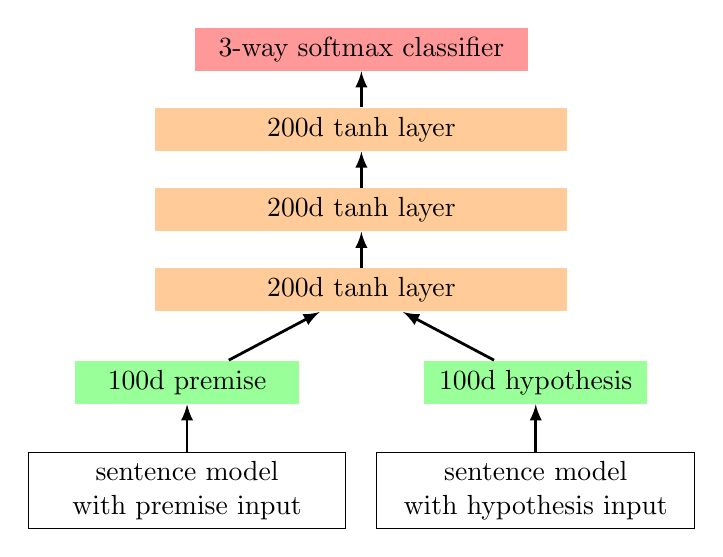
\begin{tikzpicture}
    \def\dx{21pt}
    \def\dy{29pt}

    \tikzstyle{label}=[text width=40mm,align=center]    
    \tikzstyle{softmax}=[fill=red!40,text width=40mm,align=center]
    \tikzstyle{preclass}=[fill=orange!40,text width=50mm,align=center]
    \tikzstyle{e}=[fill=green!40,text width=26mm,align=center]
    \tikzstyle{m}=[draw=black,text width=38mm,align=center]    
    
    \node[softmax]  (softmax) at (0*\dx,6*\dy) {3-way softmax classifier};
    \node[preclass]  (pc3) at (0*\dx,5*\dy) {200d $\tanh$ layer};
    \node[preclass]  (pc2) at (0*\dx,4*\dy) {200d $\tanh$ layer};
    \node[preclass]  (pc1) at (0*\dx,3*\dy) {200d $\tanh$ layer};
    \node[e]  (pe) at (-3*\dx,1.85*\dy) {100d premise};
    \node[e]  (he) at (3*\dx,1.85*\dy) {100d hypothesis};
    \node[m]  (pem) at (-3*\dx,0.5*\dy) {sentence model\\ with premise input};
    \node[m]  (hem) at (3*\dx,0.5*\dy) {sentence model\\ with hypothesis input};    
    
    \pgfsetarrowsend{latex}
    \tikzstyle{fwd} = [draw=black, line width=1pt]

          \draw [fwd] (pc3) -- (softmax);
          \draw [fwd] (pc2) -- (pc3);
          \draw [fwd] (pc1) -- (pc2);
          \draw [fwd] (pe) -- (pc1);
          \draw [fwd] (he) -- (pc1);
          \draw [fwd] (hem) -- (he);
          \draw [fwd] (pem) -- (pe);

  \end{tikzpicture}}
	
        \caption{The neural network classification architecture: for each sentence embedding model evaluated in \reftabs{tab:nnresults}{tab:transferresults}, two identical copies of the model are run with the two sentences as input, and their outputs are used as the two 100d inputs shown here.}
  \label{modelstructure}
\end{figure}

Our neural network classifier, depicted in Fig.~\ref{modelstructure} is simply a stack of three 200d $\tanh$ layers, with the bottom layer taking the concatenated sentence representations as input and the top layer feeding a softmax classifier, all trained jointly with the sentence embedding model itself.

We test three sentence embedding models, each set to use 100d phrase and sentence embeddings. Our baseline sentence embedding simply sums the embeddings of the words in each sentence. In addition, we experiment with two simple sequence embedding models models: a plain RNN and an LSTM RNN \cite{hochreiter1997long}. Both use the simple conventional layout with one layer per input token.

The word embeddings for all of the models are initialized with the 300d reference GloVe vectors (840B token version, \citealt{pennington2014glove}) and fine tuned. In addition, all of the models use an additional $\tanh$ neural network layer to map these 300d embeddings into the lower-dimensional phrase and sentence embedding space. All of the models are randomly initialized using standard techniques and trained using AdaDelta \cite{zeiler2012adadelta} minibatch SGD until performance on the development set stops improving. We applied L2 regularization to all models, manually tuning the strength coefficient $\lambda$ for each, and additionally applied dropout \cite{srivastava2014dropout} to the inputs and outputs of the sentence embedding models (though not to its internal connections) with a fixed dropout rate. All models were implemented in a common framework for this paper, and the implementations will be made available at publication time.

\begin{table}
\begin{center}
\begin{tabular}{l@{\hskip \colspaceL}@{\hskip \colspaceL}c@{\hskip \colspaceL}c}
\hline
\textbf{Sentence model} & \b{Train}  & \b{Test}\\
\hline
\t{100d Sum of words}            & \t{79.3} & \t{75.3} \\
% scr/snlirc3d-snlirc3-only-l0.0001-dim100-ed300-td3-pen200-do0.9-0.9-co3-comp-1-dp1-gc5-lstminit5/stat_log
% 290500, dev 76.4, mostly converged, but check

\t{100d RNN}            & \t{73.4} & \t{71.8} \\	
% scr/snlirc3d-snlirc3-only-l0.0001-dim100-ed300-td3-pen200-do0.9-0.9-co3-comp3-dp1-gc5-lstminit5/stat_log
% 307500, dev 71.744, 

\t{100d LSTM RNN}            & \t{84.8} & \b{78.0} \\
% scr/snlirc3d-snlirc3-only-l3e-05-dim100-ed300-td3-pen200-do0.95-0.95-co3-comp2-dp1-gc5-lstminit5/stat_log
% 372000, dev 79.039

% \t{100d TreeRNN}            & \t{69?} & \t{69?} \\
% \t{50d TreeRNTN}            & \t{61?} & \t{60?} \\
% \t{100d LSTM TreeRNN}            & \t{72?} & \t{73?} \\
\hline
\end{tabular}
\end{center}
% The caption
\caption{
\label{tab:nnresults}
Accuracy in 3-class classification on our training and test sets for each model.
}
\end{table}

The results are shown in Table~\ref{tab:nnresults}. The sum of words model performed slightly worse than the fundamentially similar lexicalized classifier---while the sum of words model is able to use pretrained word embeddings to better handle rare words, it lacks even the rudimentary sensitivity to word order that the lexicalized model's bigram features provide. Of the two RNN models, the LSTM's more robust ability to learn long-term dependencies serves it well, giving it the strongest performance of any model we tested.

\subsubsection{Evaluating on SICK}

To the extent that successfully training a neural network model on our corpus forces that model to encode broadly accurate representations of English scene descriptions, and to build an entailment classifier over those relations, we should it to be possible to trained models for use on other NLI tasks. In this section, we evaluate on the SICK task using a simple transfer learning method, and achieve competitive results.

To perform transfer, we take the parameters of strong LSTM RNN model trained on our corpus and use them to initialize new model, which trained from that point only on the training portion of SICK. The only newly initialized parameters are the embeddings for words that appear in the SICK training set, but not in our training set, and those parameters are initialized using GloVe embeddings as above. We use the same model hyperparameters that were used to train the original model, with the exception of the L2 regularization strength which is re-tuned. We additionally transfer the accumulators that are used by AdaDelta to set the learning rates. This lowers the starting learning rates, and is intended to ensure that the model does not learn too quickly in its first few epochs after transfer and destroy the knowledge accumulated in the pre-transfer phase of training.

\begin{table}
\begin{center}
\begin{tabular}{l@{\hskip \colspaceL}@{\hskip \colspaceL}c@{\hskip \colspaceL}c}
\hline
\textbf{Sentence model} & \b{Train}  & \b{Test}\\
\hline
\t{100d LSTM RNN (random init.)}            & \t{100} & \t{71.3} \\
% From: ~/quant/transfer-sick-only-l0.0001-dim50-ed200-td3-pen100-do0.9-0.9-ws1-par0-comp2-cdim1/

\t{100d LSTM RNN (transfer init.)}            & \t{99.9} & \b{80.8} \\
% From: ~/quant/transfer5-sick-only-transfer-l0.0001-dim100-ed300-td3-pen200-do0.95-0.95-ws3-adi0-comp2-cdim1/stat_log
\hline
\end{tabular}
\end{center}

\caption{\label{tab:transferresults}
The performance (\% accuracy) of an LSTM RNN model on SICK under both a random initialization and a transfer initialization copied from a model trained on our corpus.} 
\end{table}

We compare the performance of an LSTM model with both the transfer initialization and a normal random initialization. We tune the regularization parameter separately for each case. Table \ref{tab:transferresults} shows these results.

Our transfer model shows the best performance yet reported on SICK for an unaugmented neural network model, and approaches the overall state of the art at 84.6\% \cite{lai2014illinois}, as well as the 84\% level of interannotator agreement, which represents a likely performance ceiling. The randomly initialized model performs relatively poorly. This suggests that the introduction of a large high-quality corpus makes it newly possible to train representation learning models for sentence meaning of a level of quality that is competitive with the best hand-engineered models on inference tasks.

\todo{Comparison with other models on 2?3?-way SICK}

We attempted to apply this same transfer evaluation technique to the RTE-3 challenge, but found that the small size of the training set (800 examples) did not allow the model to adapt to the unfamiliar genre of text used in that corpus, such that neither our transfer model nor our randomly initialized model reached competitive performance.

\subsection{Further analysis}

Fig.~\ref{fig:bowlearncurve} shows a learning curve for the LSTM and the lexicalized and unlexicalized feature-based models. This learning curve shows that the large size of the corpus is crucial to both the LSTM and the lexicalized model, and suggests that additional data would yield still better performance for both. It is also worth noting that though the LSTM and the lexicalized model show similar performance when trained on the data we present here, the steeper slope for the LSTM suggests that its ability to learn arbitrarily structured representations of sentence meaning would give it an advantage over the more constrained lexicalized model on still larger datasets.

% useful resource in the development of more sophisticated SE models

\Fig{learning_curves_bow.pdf}{0.45}{bowlearncurve}{
A learning curve for the lexicalized and unlexicalized baseline classifiers and the LSTM,
plotted on a log scale. The minibatch-based training method that we chose for the LSTM requires at least 64 examples to function. Note that the y axis starts at a random-chance accuracy of 33\%. \todo{One more LSTM data point at ~80}}

% Insights 2: the learning curve for the unlexicalized classifier is sad
We were struck by how quickly the lexicalized classifier outperforms its unlexicalized counterpart.
With only 100 training examples, the cross-bigram classifier already outperforms its unlexicalized counterpart.
Empirically, we find that the top weighted features for the classifier
  trained on 100 examples tend to be high precision entailments;
  e.g.,
  \textit{playing} $\rightarrow$ \textit{outside}
  (most scenes are outdoors), or \textit{a banana} $\rightarrow$
  \textit{person eating}.
If relatively few spurious entailments get high weight---as it appears
is the case---then it makes sense that, when these do fire, they
boost accuracy.
  
%\todo{Insert example-specific error analysis}

There are revealing patterns in the errors common to all the models
considered here. Despite the large size of the training corpus and the
distributional information captured by GloVe initialization, many
lexical relationships are still misanalyzed, leading to incorrect
predictions of \ii{independent}, even for pairs that are common in the
training corpus like \word{beach}/\word{surf} and
\word{sprinter}/\word{runner}. Semantic mistakes at the phrasal level
(e.g., predicting contradiction for \word{A shopper buys cat food at a
  Walmart}/\word{A person shops for their pet at a stor}) indicate
that additional attention to compositional semantics would pay off.
%
% Others that could replace the above:
% \word{Two teen girls relax on a black futon}/\word{Two young girls are sitting inside}
% \word{A male is placing an order in a deli}/\word{A man buying a sandwich at a deli}
%
However, many of the persistent problems run deeper, to inferences
that depend on world knowledge and context-specific inferences, as in
the entailment pair \word{A race car driver leaps from a burning
  car}/\word{A race car driver escaping danger}, for which all our
models predict \ii{independent}. Some of these examples have qualities
reminiscent of Winograd schema \cite{Winograd:1972,Levesque:2013}. For
example, it seems likely that all the models wrongly predict
entailment for \word{A young girl throws sand toward the
  ocean}/\word{A girl can't stand the ocean}, presumably because of
distributional associations between \word{throws} and \word{can't
  stand}.




% A woman prepares ingredients for a bowl of soup.	A soup bowl prepares a woman.